\chapter{Asking Politicians How They Actually Got Rich!}

This chapter is best read as a field lecture carried out in motion. We begin outside the Capitol with refusals, hurried walk-bys, and half-finished answers; only gradually does the scene yield usable doctrine. The lecture then settles into four linked mechanisms: the acquisition of a first productive asset, the compounding of trust through service, the decade-scale accumulation behind so-called overnight success, and finally the arithmetic of debt, information, and votes inside Washington. No validated board equations survive for this lecture, so the mathematics below is deliberately schematic. Its purpose is not to replace the interviews with a false textbook, but to preserve the causal spine that the speakers themselves keep uncovering.

\section{Access Friction at the Capitol}

The lecture opens with a method before it opens with a thesis. The host asks a blunt wealth question: when did you make your first million? In another setting that might produce a neat origin story. Here it produces something else: deflection, speed, and asymmetry. People are on their way to meetings, unwilling to stop, and sometimes only after a beat does it become clear that the person hurrying past is a member of Congress. The first lesson is therefore epistemic. Washington does not hand over its mechanisms in lecture-hall form. One must first get the subject to stop.

We can summarize the opening field-method by the chain
\begin{equation}
\text{cold approach}\to \text{refusal / motion}\to \text{brief stop}\to \text{usable doctrine}.
\end{equation}
This is not decorative. It explains why the chapter must preserve the opening refusals. They are part of the lecture's argument. Politics appears first not as transparent explanation but as guarded movement.

\begin{figure}[h]
\centering
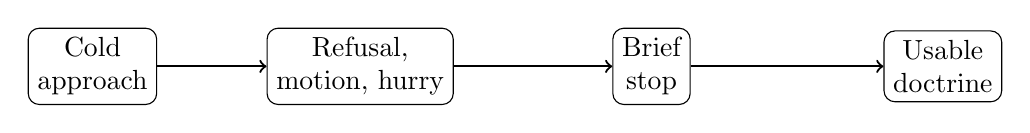
\begin{tikzpicture}
\node[draw, rounded corners, align=center] (a) at (0,0) {Cold\\ approach};
\node[draw, rounded corners, align=center] (b) at (3.4,0) {Refusal,\\ motion, hurry};
\node[draw, rounded corners, align=center] (c) at (7.1,0) {Brief\\ stop};
\node[draw, rounded corners, align=center] (d) at (10.8,0) {Usable\\ doctrine};
\draw[->, thick] (a) -- (b);
\draw[->, thick] (b) -- (c);
\draw[->, thick] (c) -- (d);
\end{tikzpicture}
\caption{The opening method of the lecture. Before we get content, we get access friction; before we get doctrine, we get motion.}
\end{figure}

Only after this teaser pressure does the host give the mission in plain form: he is in Washington, D.C.\ for the first time, trying to understand how politicians became wealthy before and perhaps after politics, and what government actors may know that ordinary people do not. That explicit frame comes after the friction, not before it. The lecture wants us to feel the difficulty of extraction before it lets us hear the answer.

\section{Mike Collins: First Asset, First Bank, First Scale}

The first strong stop is Mike Collins, and with him the lecture moves from spectacle to mechanism. The host asks about wealth in the broad sense, but Collins answers with a narrower and more useful object: the first business. He started at age $23$, in trucking, with one truck. He says he still owns that business, that it now runs over one hundred trucks a day, and that he also has a brokerage company. When the host asks about a large year, Collins gives a revenue interval rather than a precise number. We should preserve the scale without pretending to possess an audited ledger:
\begin{align}
N_{\text{trucks}} &: 1 \to 100+,\\
R_{\max} &\in [20,50]\ \text{million USD}.
\end{align}

This pair of relations already tells us something important about the lecture's logic. The visible scale is large, but the story does not begin there. The lecture insists on moving backward from the large operation to the first productive foothold.

\paragraph{Anecdote.} One truck comes first; the brokerage company and the large daily flow come later.

\paragraph{Claim.} Scale is not the starting point. It is the result of an earlier financing event and of continued execution.

\paragraph{Mechanism.} The lecture now narrows to the crucial question: how does one buy the first truck?

\subsection{Question \& Answer}

\paragraph{Question.} How does someone buy the first productive asset without inherited capital?

\paragraph{Answer.} Collins answers by going to a small community bank. More precisely, he says that the bank knew its customer, because it was part of the community. The lecture does not supply a loan rate, a collateral ratio, or a formal underwriting model, so we should not invent them. But the mechanism itself is clear enough to write:
\begin{equation}
\text{local bank knowledge}\to \text{credit}\to \text{first truck}\to \text{operating revenue}\to \text{scale}.
\end{equation}
The point is not sentimentality about small banks. The point is informational. A lender with local knowledge does not face the same kind of abstraction as a distant institution. The first asset is therefore financed not by generic confidence, but by knowledge tied to a place and a person.

\begin{figure}[h]
\centering
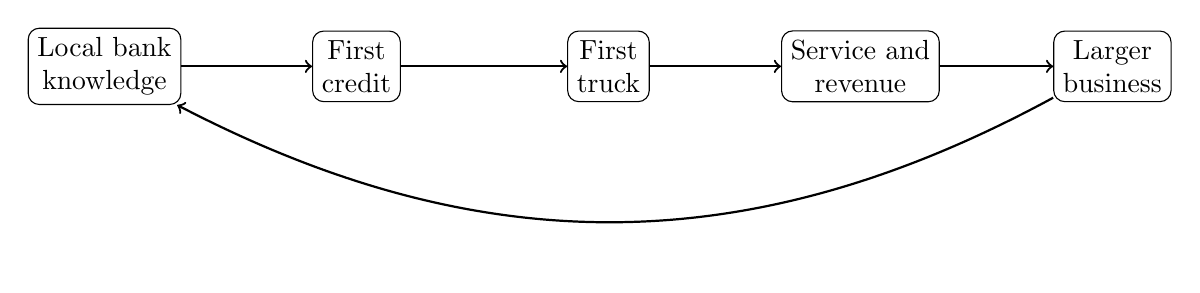
\begin{tikzpicture}
\node[draw, rounded corners, align=center] (a) at (0,0) {Local bank\\ knowledge};
\node[draw, rounded corners, align=center] (b) at (3.2,0) {First\\ credit};
\node[draw, rounded corners, align=center] (c) at (6.4,0) {First\\ truck};
\node[draw, rounded corners, align=center] (d) at (9.6,0) {Service and\\ revenue};
\node[draw, rounded corners, align=center] (e) at (12.8,0) {Larger\\ business};
\draw[->, thick] (a) -- (b);
\draw[->, thick] (b) -- (c);
\draw[->, thick] (c) -- (d);
\draw[->, thick] (d) -- (e);
\draw[->, thick, bend left=28] (e) to (a);
\end{tikzpicture}
\caption{A cautious transcript-derived reconstruction of the Collins mechanism. Successful execution feeds back into future creditworthiness and reputation.}
\end{figure}

At once the lecture does something characteristic. Having given the first-asset story, it refuses to remain merely anecdotal. Collins uses the story to widen outward: community banks have been decimated, local credit has been thinned out, and the disappearance of that layer changes what becomes possible for the next entrant. The host then keeps tugging the conversation back toward concrete business logic rather than letting it dissolve into slogan.

\section{From Local Credit to Service and Incentive}

Once the first truck is in place, Collins turns from finance to differentiation. The trucking business is competitive. The host asks directly what allowed Collins to stand out. The answer is not bigness, and it is not even ``hard work'' in the abstract. The answer is service: do what you say you will do, and when something goes wrong, compensate, repair, and keep the customer whole.

That suggests a trust update rule:
\begin{equation}
T_{t+1}=T_t+\Delta T_t,\qquad \Delta T_t>0,
\end{equation}
where $\Delta T_t$ is the trust increment generated by one fulfilled commitment, or by one disruption competently repaired.

If we write the increments as $\delta_1,\delta_2,\dots,\delta_n$, then the recurrence unfolds in the usual way:
\begin{align}
T_1 &= T_0+\delta_1,\\
T_2 &= T_1+\delta_2 = T_0+\delta_1+\delta_2,\\
T_n &= T_0+\sum_{i=1}^n \delta_i.
\end{align}
This is the most useful worked mathematics in the Collins section. The firm need not be the largest in the field. It needs a positive stream of reliability increments. That stream changes future demand. Customers call back not because the firm is maximal, but because the trust stock is nontrivial.

The lecture then lifts the same pattern into politics. Collins says that people reward delivery there too, and points to his record of having bills signed under presidents of different parties. We should not collapse business and government into the same thing, but the analogy is deliberate: repeated visible performance alters future willingness to deal with you.

The other widening move in this section concerns incentive. Collins insists that the free market works and that small business matters because it preserves the incentive to start from the ground up, take risk, and work upward. Here again we should distinguish speaker claim from reconstructed mechanism. The claim about political parties and administrations remains his. The stable mechanism is simpler: if upside can still be retained, then risk-taking remains intelligible to the builder.

\subsection{Question \& Answer}

\paragraph{Question.} Is hard work by itself enough?

\paragraph{Answer.} Not in the form this lecture gives it. Hard work is necessary, but it becomes economically visible only when it is attached to delivery. Pure exertion is not yet a commercial asset. Repeated service, by contrast, enters the recurrence for $T_t$ and changes the future call pattern. In the lecture's own cadence, the distinction is exact: work hard, yes; but then do what you say, again and again.

The host then gives a brief recap outside the Capitol. This reset matters. Washington remains refusal-heavy terrain. The lecture does not want one strong interview to swallow the whole field, so it steps back, reasserts the strangeness of the setting, and goes back into the hunt.

\section{Gregory Meeks: Education, Reading, and Civic Trajectory}

The next strong stop shifts the lecture onto a different line of ascent. Gregory Meeks does not begin with a business scale story. He begins with public housing, poverty, and the obligation to contribute. The host asks what changed the family's trajectory. Meeks answers with an ordered path: education first, family next, then reading, then awareness of the surrounding environment, and then the decision to make a difference.

The sequence is structural enough to be preserved as a state progression:
\begin{equation}
\text{public housing}\to
\text{education}\to
\text{reading}\to
\text{environment awareness}\to
\text{contribution}\to
\text{office}.
\end{equation}
This is not a quantitative mobility model, and it should not be presented as one. Its value lies elsewhere. It shows that the lecture is broadening its notion of wealth and ascent. The route to a consequential life is not only first company, first truck, first scale. It can also be first book, first awareness, first decision to contribute.

There is also a useful rarity marker in the exchange. Meeks remarks that there are only about five hundred or so people in the House of Representatives:
\begin{equation}
N_{\text{House}}\approx 500.
\end{equation}
We should leave the count in this approximate form, because the lecture uses it as a scale marker, not as a civics exercise. The point is that office is rare, and the path into it is therefore a path into a very small institutional set.

\subsection{Question \& Answer}

\paragraph{Question.} What is the first actionable step in changing a family's trajectory?

\paragraph{Answer.} In this lecture the answer is ordered, not mystical: education first, then reading, then awareness, then contribution. That order is part of the argument. It prevents the story from dissolving into generic uplift.

The Meeks interview then widens in its own way. Faith appears not primarily as explanation of unexpected openings, but as decision-making orientation. He speaks about the Bible, about Dr.\ King, and about trying to do what is right, humane, and godly. From there the host raises a tension that has hovered since the beginning: if politics is a nasty game, why enter it at all? Meeks answers that politics is precisely how things are changed, and that the civil-rights movement created the right for him to stand there in the first place. The lecture therefore offers a second non-monetary interpretation of office: not enrichment, but inherited obligation.

Finally, the interview turns again toward life-form rather than institution. Meeks speaks about taking care of the body, and then about self-belief and purpose. That last move is important because it prepares the lecture's closing pattern: the public and the personal will not remain separate for long.

\section{The Montana Route: Startup, Yahoo, and the Decade Game}

After another recap and another return to the street, the lecture swings back toward classical entrepreneurship. The representative from Montana offers the most recognizably startup-shaped route in the episode: poor origin, college, success there, work at New York University as a research scientist, teaching, then a startup merged with Yahoo by a pooling-of-interests transaction, and then angel financing and early-stage technology work. After September 11 he joins the Air Force, serves in Afghanistan, and later carries all of that into Congress.

We should preserve the route without pretending to know the cap table. The lecture gives a merger structure and a share-pooling description; it does not give ratios. What it does give, very cleanly, is the doctrine that follows: the secret of overnight success is to keep turning the crank.

That doctrine admits a natural recurrence:
\begin{equation}
B_{t+1}=B_t+\Delta B_t,\qquad \Delta B_t>0
\end{equation}
under continued execution.

Over many periods,
\begin{equation}
B_n=B_0+\sum_{i=0}^{n-1}\Delta B_i.
\end{equation}
This is a useful place to slow down and read the lecture carefully. The speaker is not merely praising perseverance in a moral sense. He is drawing attention to accumulation itself. What looks sudden at the end is, in ordinary cases, the terminal visibility of a long sum.

The host notices this immediately and restates it in the right language: decades, not short term. The Montana speaker agrees. One keeps pushing the ball forward, keeps showing up, and eventually looks behind and sees that something large exists.

The lecture sharpens the point with a work-intensity anchor from the speaker's early technology years:
\begin{equation}
h_{\text{work}}\approx 20\ \text{hours/day},\qquad s_{\text{sleep}}\approx 4\ \text{hours/night}.
\end{equation}
These are self-reported magnitudes, not prescriptions. Their function is to strip away the glamour of the end state and recover the input pattern.

\subsection{Question \& Answer}

\paragraph{Question.} Why does ``overnight success'' still require decades?

\paragraph{Answer.} Because the visible result is a snapshot and the real process is cumulative. The lecture's own formulation is almost mechanical: keep turning the crank. In notation, the built object after many periods is the sum of many increments, not the result of one theatrical jump.

This interview then makes a significant turn. Having narrated his private path, the speaker immediately asks what kind of America still exists for the next entrant. He worries about fiscal looseness, about the increasing distance to a first home, and about whether ordinary families or small-business starters still have a genuine path upward. That political pivot is not an afterthought. It is the bridge to the final and sharpest segment of the lecture.

\section{Byron Donalds: Debt Arithmetic and Insider Asymmetry}

Byron Donalds brings the most explicit fiscal language. His route into politics begins in finance, with research done during the 2008 crisis. He did not dream from childhood of holding office; rather, political engagement emerged out of trying to understand what was happening to the economy.

From there the lecture states a compact sequence. One cannot borrow forever. The more money is borrowed, the more it costs. Higher national debt destroys purchasing power, and the first people harmed are poor households and seniors on fixed incomes. A cautious schematic version is
\begin{equation}
D'(t)>0 \Rightarrow \text{cost burden rises} \Rightarrow P_{\text{pp}}(t)\downarrow,
\end{equation}
where $D(t)$ denotes the debt path and $P_{\text{pp}}(t)$ denotes the purchasing power available to ordinary Americans. This is not a calibrated macroeconomic law. It is a transcript-faithful statement of direction.

\subsection{Question \& Answer}

\paragraph{Question.} If borrowing cannot stop immediately, what does it mean to slow the trajectory first?

\paragraph{Answer.} The distinction is between level and slope. The debt stock may still be rising while the rate at which it rises is reduced:
\begin{equation}
D'_{\text{slowed}}(t)<D'_{\text{current}}(t),
\end{equation}
even if both derivatives remain positive for a while.

Over a horizon $T$, the separation between the two paths is
\begin{equation}
D_{\text{current}}(T)-D_{\text{slowed}}(T)
=
\int_0^T \bigl(D'_{\text{current}}(t)-D'_{\text{slowed}}(t)\bigr)\,dt.
\end{equation}
If that integrand stays positive, the gap widens. This is the precise content of the phrase ``slow the trajectory.'' It does not yet mean paydown. It means that before we reverse the path, we first reduce its steepness.

\begin{figure}[h]
\centering
\begin{tikzpicture}
\draw[->] (0,0) -- (6.6,0) node[right] {$t$};
\draw[->] (0,0) -- (0,4.6) node[above] {$D(t)$};
\draw[thick] (0.4,0.5) .. controls (2,1.0) and (4,2.1) .. (6.1,4.0);
\draw[thick] (0.4,0.5) .. controls (2,0.9) and (4,1.6) .. (6.1,2.9);
\node at (5.1,3.85) {$D_{\text{current}}$};
\node at (4.9,2.55) {$D_{\text{slowed}}$};
\end{tikzpicture}
\caption{A transcript-derived borrowing picture. Both paths may rise at first; the immediate aim is to reduce the slope before any later paydown.}
\end{figure}

Donalds then moves into ethics. Members of Congress, he says, possess information that ordinary people do not. The notation is minimal but useful:
\begin{equation}
I_{\text{member}} > I_{\text{public}}.
\end{equation}
From this he does not infer a theorem about market efficiency. He infers an ethical problem. If that asymmetry exists, then direct member trading is compromised. He therefore delegates trading to a firm and says explicitly that he thinks it is unethical for members to trade on their own account while holding office.

A caution is necessary here. The transcript contains a likely unstable numerical fragment when the conversation turns to famous political wealth. The lecture clearly wants to point to highly visible cases of enrichment, but the exact number in the transcript is too noisy to be mathematized. The mechanism, however, does not depend on that number. It depends only on the asymmetry $I_{\text{member}} > I_{\text{public}}$ and on the moral conclusion Donalds draws from it.

The section closes with a vivid date marker. Asked when he first understood Washington, he says that his third day there was January 6, shortly after being sworn in. The lecture does not analyze that event statistically. It uses it as a scene of institutional immediacy. The student of these notes should feel the sequence: finance background, debt arithmetic, trading ethics, then immediate immersion into the raw stress of the institution itself.

\section{Fear, Votes, and the Person Behind the Office}

Once the lecture has established debt and insider asymmetry, it moves deeper into the institution. What would shock people, Donalds says, is how afraid most members are: afraid of criticism, afraid of the tough choice, afraid of doing now what would be best later. This leads naturally to the question of who really holds power in Washington.

His answer begins with the obvious offices---the president, the Speaker, the Senate majority leader---and then turns sharply to a better operational rule. Real power belongs to a cluster of members willing to stand firm, because in the end everyone is counting votes. The arithmetic can be written plainly:
\begin{equation}
V\ge V_{\text{majority}} \Rightarrow \text{floor action},\qquad
V<V_{\text{majority}} \Rightarrow \text{stasis}.
\end{equation}
This is one of the lecture's most useful clarifications. It distinguishes title from effective control. In a legislative chamber, power is often nothing more mysterious than coalition size at the decisive moment.

The lecture then makes the same move morally. If power can corrupt, then long indefinite occupancy becomes dangerous; hence Donalds's support for term limits. Again, the lecture does not give a formal theory of institutional decay, but it does give a direction: one should not stay forever, and one should eventually go home.

From there the interview becomes strikingly personal. Donalds recalls the toughest decision of his political life in the context of being nominated for Speaker. He describes prayer, a call to his wife, a sense of the gravity of the moment, and then the public test that followed. The point of the anecdote is not theatrical self-display. It is that institutional choice is experienced by an actual person under pressure, not by a diagram alone.

The next movement is a life-course heuristic. A boss told him at age $29$ to get to where he wanted to get by age $40$, because that is when money and mark really start to compound:
\begin{equation}
a_{\text{advice}}=29,\qquad a_{\text{target}}=40.
\end{equation}
We should read this as guidance, not law. The transcript uses it to distinguish the grind years from the years of visible compounding.

Finally the lecture reaches its cleanest threshold. Donalds speaks about arrests at $18$ and $20$, and then about a decision at $20$ that he would never be in that position again. The right mathematical form is not a gradual drift, but a state change:
\begin{equation}
S_{20^-}\xrightarrow{\text{decision at }20} S_{20^+}.
\end{equation}
The force of the passage lies precisely in that discreteness. A life can contain slow compounding, but it can also contain a gate.

Faith then stabilizes the new path. He gives his life to Christ at $21$, later recounts the Cracker Barrel conversion scene, and frames the subsequent years as guidance rather than victimhood. By the time the host asks whether the system is rigged, the lecture has already prepared the answer. Donalds says people are missing the playbook. The sentence should not be read as a denial of structure; the chapter has just spent pages on structure. It should be read as a refusal of paralysis.

\subsection{Question \& Answer}

\paragraph{Question.} What changes first: the system around us, or the decision we make in the mirror?

\paragraph{Answer.} The lecture answers in two steps. Public structures matter enormously: debt paths matter, information asymmetries matter, vote thresholds matter. But transition into agency still begins with a decision. One decides, then one works, then one compounds. The public and the private are therefore not rival explanations here. They are sequentially braided.

\section{Summary}

The lecture begins in motion and ends in structure. First we learn that Washington is a refusal-heavy field in which doctrine must be extracted in transit. Then Collins gives the first productive-asset mechanism: one truck, one community bank, and eventually scale. From there the lecture turns to service, where repeated delivery raises a stock of trust and changes future demand. Meeks then widens the picture by giving a different ladder: education, reading, awareness, contribution, office. The Montana interview returns to entrepreneurship, but now in its properly long horizon: a startup route, a Yahoo merger, and the recurrence behind ``turning the crank.'' Finally Donalds gives the sharpest arithmetic of the episode: debt slope, purchasing power, insider-information ethics, coalition votes, career compounding, and the threshold act by which a life changes course.

What remains is not a single formula for wealth. It is a linked set of mechanisms. Productive assets matter. Local knowledge matters. Repeated service matters. Time matters. Public debt is not abstract if it reaches down into household purchasing power. Office is not the same thing as power if votes are missing. And the person moving through such a system is still, at decisive moments, the person who must decide what sort of life to lead.